\section{Simmetria \PT\ e \CPT}
\begin{frame}{Operatori \PT-invarianti}
    Diciamo che un operatore è \hPT-invariante se
    $$\PTtransform{\hA} = \hA\mycomma$$
    o analogamente
    $$\comm*{\hPT}{\hA}\! = 0\myperiod$$
    \pause
    Se $\ket{\psi}$ è un autostato \emph{simultaneo} di \hA\ e \hPT, l'autovalore $\lambda$ di \hA\ associato a $\ket{\psi}$ è \emph{reale}, infatti
    \begin{align*} 
        \hPT\pqty*{\hA\!\ket{\psi}}\! = \hPT\pqty{\lambda\!\ket{\psi}}
        \quad&\iff\quad
        \pause
        \hA\hPT\!\ket{\psi} = \lambda^*\hPT\!\ket{\psi} \\
        \pause
        \hA\!\ket{\psi} = \lambda^*\!\ket{\psi}
        \quad&\iff\quad
        \lambda\!\ket{\psi} = \lambda^*\!\ket{\psi}
    \end{align*}
\end{frame}

\begin{frame}
    Domanda:
    \begin{center}
        {\it Esiste una classe più generale di operatori con autovalori reali?}
    \end{center}
    Risposta:
    \pause
    \begin{center}
        {\it Sì e no, perché non tutti gli operatori Hermitiani sono \emph{anche} \PT-invarianti, ma esistono operatori \emph{non Hermitiani} che hanno autovalori reali.}
    \end{center}
    \pause
    \begin{figure}
        \centering
        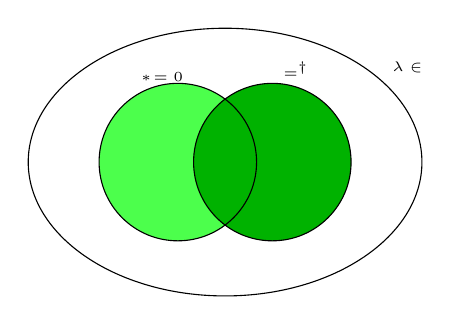
\begin{tikzpicture}
            \fill[color=green!70!white] (-0.6,0) circle (1);
            \fill[color=green!70!black] (0.6,0) circle (1);
            \draw (-0.6,0) circle (1);
            \draw (+0.6,0) circle (1);
            \draw (0,0) ellipse (2.5 and 1.7);
            \node[anchor=south] at (0.9,0.95) {\tiny{$\hH = \hH^\dag$}};
            \node[anchor=south, align=center] at (-0.8,0.9) {\tiny{$\comm*{\hPT}{\hH}\! = 0$}};
            \node[anchor=west, align=center] at (2,1.2) {\tiny{$\lambda\in\bbR$}};
        \end{tikzpicture}
    \end{figure}
\end{frame}

\begin{frame}{Simmetria \PT}
    Diciamo che un sistema fisico \emph{non rompe la Simmetria \PT} se
    \begin{enumerate}[label=\mybullet]
        \pause
        \item L'Hamiltoniana \hH\ commuta con \hPT;
        \pause
        \item Gli autostati di \hH\ sono simultaneamente autostati di \hPT.
    \end{enumerate}
    \pause
    In questo caso lo spettro di \hH, ovvero le possibili misure di energia, sono reali.
\end{frame}

\begin{frame}
    Una nuova domanda:
    \begin{center}
        {\it Possiamo costruire una teoria quantistica a partire da Hamiltoniane \PT-invarianti?}
    \end{center}
\end{frame}

\begin{frame}{Ci siamo persi qualcosa...}
    Quali sono le proprietà fondamentali di cui una teoria quantistica non può fare a meno?
    \begin{enumerate}
        \pause
        \item[\ding{51}] Le misure devono essere numeri reali;
    \end{enumerate}
    \pause
    inoltre, nello spazio di Hilbert deve essere definito un prodotto interno tale che
    \begin{enumerate}
        \pause
        \item[\ding{55}] Gli autospazi siano ortogonali;
        \pause
        \item[\ding{55}] La probabilità si conservi;
    \end{enumerate}
    \pause
    Senza farci caso abbiamo perso le ultime due proprietà.
\end{frame}
